\chapter{Choosing a Transformer-based Toxicity Analyzer} \label{choosing-toxicity-analyzer}
Modern toxicity detection systems rely on Transformer-based architectures like BERT \cite{devlin:2019}, which analyze entire sentences to capture word relationships. This capability helps identify toxic language patterns that depend on context. Our study evaluates three Transformer-based models, including one enhanced with a Convolutional Neural Network. BERT's bidirectional training approach, learning from both surrounding words, enables detection of subtle toxic content like sarcasm or coded expressions \cite{mathew:2021}.

To analyze the toxicity of toots, we choose one of those three models: Detoxify (Original), Detoxify (Unbiased) from Unitary, and Perspective API. These models predict probabilities for six to seven toxicity categories.

\textbf{Detoxify Original}\footnote{\url{https://huggingface.co/unitary/toxic-bert}} is trained on English text using the "Jigsaw Toxic Comment Classification Challenge" dataset, which comprises Wikipedia comments. The model predicts probability scores for toxicity labels, which include categories similar to those listed in Table~\ref{toxicity-categories}, but without the sexually explicit label. The model is based on the BERT-base-uncased transformer architecture and fine-tuned on the Jigsaw dataset. During prediction, the input text is tokenized and processed through the transformer model to generate the output scores \cite{detoxify:medium}.

\textbf{Detoxify Unbiased}\footnote{\url{https://huggingface.co/unitary/unbiased-toxic-roberta}} also focuses on English text but is trained on the "Jigsaw Unintended Bias in Toxicity Classification" dataset. This dataset consists of comments from "Civil Comments" platform and includes additional labels for identities to reduce bias across different demographic groups. The labels align with those in Table~\ref{toxicity-categories}. The model employs the RoBERTa-base~\cite{liu:2019} transformer architecture and is fine-tuned on the Jigsaw dataset. Like Detoxify Original, it tokenizes input text and processes it through the transformer model to produce probability scores for the labels \cite{detoxify:medium}.

\textbf{Perspective API} supports multiple languages and addresses the challenge of limited forum data for some languages by using machine translation. Labeled English-language comments are translated into the target language to supplement training data. The training dataset is sourced from diverse platforms, including Wikipedia and The New York Times, with each comment annotated by 3--10 crowdsourced raters. The labels match those in Table~\ref{toxicity-categories}. The training process begins with multilingual BERT-based models trained on the dataset, which are then distilled into single-language Convolutional Neural Networks (CNNs) for each supported language. As well as the two Detoxify models, the Perspective API outputs probability scores for the toxicity labels \cite{lees:2022}.

\begin{table}[tb]
    \centering\small
    \renewcommand{\arraystretch}{1.3}
    \begin{tabularx}{\textwidth}{lX}
        \toprule
        \textbf{Category} & \textbf{Description} \\
        \midrule
        TOXIC & A rude, disrespectful, or unreasonable comment that is likely to make someone leave a discussion. \\
        SEVERE TOXIC & A very hateful, aggressive, disrespectful comment or otherwise very likely to make a user leave a discussion or give up on sharing their perspective. \\
        IDENTITY ATTACK & Negative or hateful comments targeting someone because of their identity. \\
        INSULT & Insulting, inflammatory, or negative comments towards a person or a group of people. \\
        OBSCENE & Swear words, curse words, or other obscene or profane language. \\
        THREAT & Describes an intention to inflict pain, injury, or violence against an individual or group. \\
        SEXUALLY EXPLICIT & Contains references to sexual acts, body parts, or other lewd content. \\
        \bottomrule
    \end{tabularx}
    \caption[perspectiveapi]{Toxicity categories and their descriptions. The definitions are based on the Perspective API documentation\footnotemark.}
    \label{toxicity-categories}
\end{table}
\footnotetext{\url{https://developers.perspectiveapi.com/s/about-the-api-attributes-and-languages}}

\section{Mastodon Toots Annotation} \label{annotation}
All models were evaluated on a subset of the dataset. The selected timeframe was the evening of the 2024 Paris Olympic Games' opening ceremony, chosen due to the expectation of heightened online discussions and increased toxic content. The dataset covers the period from 20:00 to 23:00 on July~26, 2024, comprising 1,179,897 toots. This shift from general social media discourse to event-driven conversations (specifically, the Olympics' opening ceremony) may impact model performance, but simultaneously tests the models' adaptability to new context.

First, each model predicted toxicity scores for all toots in the subset. After predictions were completed, we drew a sample for each model, selecting 25 toots per toxicity category with a predicted probability greater than 0.5. The selected toots were then concatenated across models, and duplicates were removed, resulting in a final annotation dataset of 253 unique toots for human evaluation.

The annotation process was performed by two researchers using Label Studio\footnote{\url{https://labelstud.io/}}, an open-source data labeling platform. The toots were labeled according to the categories in Table~\ref{toxicity-categories}. Hate speech annotation is highly subjective and influenced by annotator biases, affecting consistency and reliability. To ensure reliability, inter-annotator agreement was measured using Cohen's Kappa. The results showed perfect agreement (Cohen's Kappa = 1.0) for the categories toxic, severe toxic, threat, insult, and identity attack. Near-perfect agreement was achieved for obscene (Cohen's Kappa = 0.9907) and sexually explicit (Cohen's Kappa = 0.9735), indicating high consistency between annotators. In cases where toots were labeled diffrently, we reviewed them and agrred on one label. For the small number of cases with divergent annotations, the researchers conducted a consensus review to resolve discrepancies and assign a final unified label.

\section{Transformer-based Model Evaluation} \label{evaluation}
The evaluation focused on the probability distributions of toxicity categories and the F1 scores across three models: Perspective API, Detoxify (Original), and Detoxify (Unbiased). A fixed threshold of 0.5 was used to predict whether a toot is toxic. The Perspective API model generally outperformed the Detoxify models in F1 scores for most categories (see Table~\ref{table-performance-metrics}).

We used the weighted average F1 score to compare the overall performance of the models because the label distribution in our subset was highly unbalanced. The Perspective API achieved a weighted average F1 score of 0.621, outperforming Detoxify Original (0.575) and Detoxify Unbiased (0.589). Notably, while the Detoxify Unbiased model performed poorly on the "severe toxic" category, its weighted average F1 score improved to 0.611 when this category was excluded. This result brings it closer to the Perspective API model, which achieved 0.636 under the same conditions.

However, the probability distributions (Figure~\ref{probability-distribution}) revealed behavioral differences. The Perspective API model exhibited a widely spread distribution, suggesting cautious predictions, while the Detoxify models showed concentrated distributions, indicating higher confidence.

\begin{figure}[tb]
    \centering
    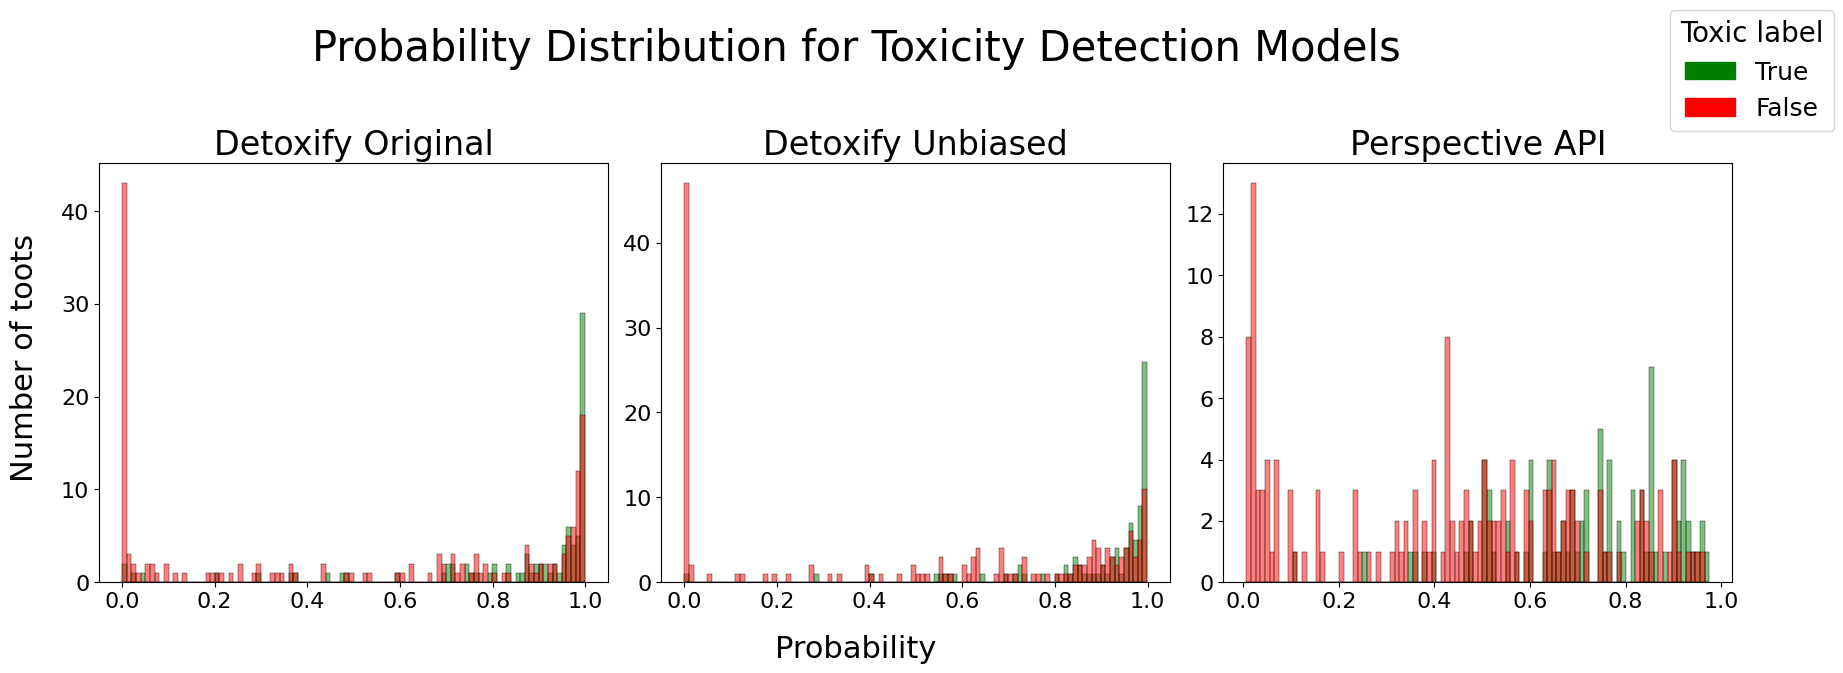
\includegraphics[width=\textwidth]{../material/probability_distribution.png}
    \caption{Probability Distribution of the toxic category across the three models}
    \label{probability-distribution}
\end{figure}

The Perspective API model's limited accessibility, due to low request rates and lack of open access, posed practical constraints for large-scale analysis. In contrast, the open-source Detoxify models offered unrestricted usage, making them more suitable for large-scale studies. The Detoxify models were ultimately selected as they align better with our research objectives: their open-source nature enables large-scale analysis of toxicity trends, while their consistent confidence scores provide more reliable tracking of toxicity patterns over time.

Between the two Detoxify models, the unbiased version was selected for further analysis due to its superior performance (Table~\ref{table-performance-metrics}) and inclusion of the "sexual explicit" category, absent in the original model. However, the "severe toxic" label in the unbiased model performed poorly, likely due to limited supporting toots (only 10 in the dataset). Findings for this category should be interpreted cautiously. Despite this, the Detoxify unbiased model was chosen for analyzing Mastodon toxicity trends, balancing performance, accessibility, and practicality.

\begin{table}[p]
    \centering\small
    \caption{Performance metrics across toxicity categories with highest F1 scores highlighted.}
    \label{table-performance-metrics}
    \begin{tabular}{@{}lrrrr@{}}
      \toprule
      \textbf{Model} & \textbf{F1} & \textbf{Precision} & \textbf{Recall} & \textbf{Support} \\
      \midrule
      \multicolumn{5}{c}{\bfseries toxic} \\
      Detoxify Original      & 0.622 & 0.482 & 0.878 & 90 \\
      Detoxify Unbiased      & 0.635 & 0.473 & 0.967 & 90 \\
      Perspective API        & \textbf{0.664} & 0.526 & 0.900 & 90 \\
      \addlinespace[0.5em]
      
      \multicolumn{5}{c}{\bfseries severe toxic} \\
      Detoxify Original      & 0.148 & 0.118 & 0.200 & 10 \\
      Detoxify Unbiased      & 0.000 & 0.000 & 0.000 & 10 \\
      Perspective API        & \textbf{0.222} & 0.176 & 0.300 & 10 \\
      \addlinespace[0.5em]
      
      \multicolumn{5}{c}{\bfseries obscene} \\
      Detoxify Original      & \textbf{0.741} & 0.613 & 0.936 & 78 \\
      Detoxify Unbiased      & 0.739 & 0.642 & 0.872 & 78 \\
      Perspective API        & 0.738 & 0.615 & 0.923 & 78 \\
      \addlinespace[0.5em]
      
      \multicolumn{5}{c}{\bfseries threat} \\
      Detoxify Original      & 0.462 & 0.429 & 0.500 & 18 \\
      Detoxify Unbiased      & 0.520 & 0.406 & 0.722 & 18 \\
      Perspective API        & \textbf{0.596} & 0.483 & 0.778 & 18 \\
      \addlinespace[0.5em]
      
      \multicolumn{5}{c}{\bfseries insult} \\
      Detoxify Original      & 0.377 & 0.312 & 0.476 & 42 \\
      Detoxify Unbiased      & \textbf{0.500} & 0.378 & 0.738 & 42 \\
      Perspective API        & 0.487 & 0.384 & 0.667 & 42 \\
      \addlinespace[0.5em]
      
      \multicolumn{5}{c}{\bfseries identity attack} \\
      Detoxify Original      & 0.440 & 0.314 & 0.733 & 15 \\
      Detoxify Unbiased      & \textbf{0.545} & 0.414 & 0.800 & 15 \\
      Perspective API        & 0.456 & 0.310 & 0.867 & 15 \\
      \addlinespace[0.5em]
      
      \multicolumn{5}{c}{\bfseries sexually explicit} \\
      Detoxify Original      & 0.000 & 0.000 & 0.000 & 21 \\
      Detoxify Unbiased      & 0.392 & 0.333 & 0.476 & 21 \\
      Perspective API        & \textbf{0.576} & 0.447 & 0.810 & 21 \\
      \addlinespace[0.5em]
      
      \cmidrule(l){1-5}
      \addlinespace[0.1em]
      \cmidrule(l){1-5}
      \multicolumn{5}{c}{\bfseries Weighted Average F1} \\
      \multicolumn{5}{c}{Detoxify Original: 0.575* \quad Detoxify Unbiased: 0.589 \quad Perspective API: \textbf{0.621}} \\
      \addlinespace[0.5em]

      \bottomrule
    \end{tabular}

    \vspace{0.2cm}
    \footnotesize *Calculated excluding the sexually explicit category as the Detoxify Original model doesn't predict this label.
\end{table}